\documentclass[12pt,a4paper]{article}
\usepackage[utf8]{inputenc}
\usepackage{amsmath}
\usepackage{amsfonts}
\usepackage{amssymb}
\usepackage{graphicx}
\usepackage{polski}
\usepackage{mathtools}
\usepackage[T1]{fontenc}
\usepackage{pdflscape}
\usepackage{graphicx}
\usepackage{caption}
\usepackage{subcaption}
\usepackage{floatrow}
\usepackage{float}
\usepackage{hyperref}
\usepackage{listings}
\usepackage{verbatim}
\DeclarePairedDelimiter{\ceil}{\lceil}{\rceil}

\newcommand{\ImgPath}{./img/}
%\Figure{filename}{caption}{label}.
%\Figure{sciezka-do-pliku.png}{Opis opis}{labelka}
\newcommand\Figure[4][width=\linewidth]{%
  \begin{figure} [h!]
    \centering
    \includegraphics[#1]{\ImgPath /#2}
    \caption{#3}\label{#4}
  \end{figure}
}

\title{Rozmieszczanie kamer bezpieczeństwa}
\author{Wiktor Franus \\ Grzegorz Staniszewski}

\begin{document}
\maketitle
\tableofcontents

\newpage
\section{Treść zadania}
Jak optymalnie rozmieścić kamery monitoringu w ustalonym pomieszczeniu (rzut z góry), aby minimalną liczbą kamer móc obserwować dowolne miejsce (z uwzględnieniem maksymalnej dopuszczalnej odległości od kamery). W rozwiązaniu należy uwzględnić możliwość zapewnienia parametryzowanej redundancji - tzn. wymagania, aby każde miejsce było obserwowane przez co najmniej $n$ kamer.

\section{Założenia}
\begin{enumerate}

\item Pomieszczenie jest wielokątem zawierającym tylko kąty o mierze 90 lub 270 stopni. 
Pomieszczenie reprezentowane jest przez zbiór punktów (z I ćwiartki układu współrzędnych) podanych w formie listy. 
Połączenie tych punktów linią, zgodnie z ich kolejnością na liście, skutkuje otrzymaniem linii łamanej ograniczającej pomieszczenie.
Punkty podawane są w kolejności zgodnej z ruchem wskazówek zegara.
Pierwszy i ostatni punkt jest taki sami (należy domknąć pomieszczenie).
\item Kamery mają jednakowy zasięg reprezentowany przez kwadrat o parametryzowanej długości boku. 
Współrzędne kamery są jednocześnie współrzędnymi środka tego kwadratu. 
Kamera musi znajdować się wewnątrz pomieszczenia i nie przenika przez ściany.
\item Wnętrze pomieszczenia zdyskretyzowane jest do zbioru punktów o współrzędnych całkowitych poprzez nałożenie siatki o parametryzowanej gęstości.
\item Punkty leżące na krawędziach wielokąta opisującego pomieszczenie nie należą do jego wnętrza.
\end{enumerate}

\section{Przestrzeń przeszukiwań}
\begin{itemize}
	\item Elementem przestrzeni przeszukiwań jest wektor par liczb całkowitych oznaczających współrzędne kamer:\\
	$$[(x_1, y_1), ..., (x_i, y_i), ..., (x_k, y_k)]$$
	gdzie:\\
	$x_i$ - współrzędna x i-tej kamery,\\
	$y_i$ - współrzędna y i-tej kamery,\\
	$k$ - liczba kamer.
	\item Przejście do sąsiedniego elementu możliwe jest poprzez:
	\begin{itemize}
		\item zmianę położenia jednej z kamer na 2 sposoby (sposób
		ustalany jest na początku zadania):
		\begin{itemize}
		\item zmiana współrzędnych x lub y jednej z kamer o 1 jednostkę,
		\item przeniesienie jednej z kamer do innego punktu z wnętrza pomieszczenia
		wylosowanego zgodnie z rozkładem jednostajnym,
		\end{itemize}
		\item dodanie nowej kamery w losowym miejscu (rozkład jednostajny),
		\item usunięcie jednej kamery.
	\end{itemize}
	\item Przestrzeń ma strukturę grafową, w której każda krawędź odpowiada
	jednemu z wymienionych wyżej przejść między elementami przestrzeni.
\end{itemize}

\section{Funkcja celu}
Informacje znane dla danej instancji problemu: \\
$n_{kmin}$ - minimalna teoretyczna liczba kamer wymagana do pokrycia danego pomieszczenia
(obliczana jako stosunek pola powierzchni pomieszczenia do pola powierzchni zasięgu jednej kamery, zaokrąglany do jedności w górę),\\
$X$ - zbiór punktów reprezentujących wnętrze pomieszczenia. \\
%
\newline
Parametry funkcji celu: \\
$\alpha$ - zysk z pokrywania powierzchni pomieszczenia,\\
$\beta$ - koszt użycia nadmiarowej kamery, \\
$r_{min}$ - minimalna liczba kamer pokrywająca każde miejsce w pomieszczeniu. \\
%
\newline
Zadanie polega na maksymalizacji funkcji: \\
$$f(p, k, r) = \alpha * p - \beta * k - \frac{1}{r_{min}} * r $$ 
gdzie: \\
$p$ - stosunek powierzchni pokrytej przez kamery do powierzchni pomieszczenia \\
$k$ - stosunek nadwyżki liczby kamer do $n_{kmin}$, obliczany wg. wzoru: \\
\indent $k = \frac{max(0, n_k - n_{kmin})}{n_{kmin}}$, gdzie $n_k$ - liczba kamer w aktualnym stanie \\\\
Parametr $r$ może być obliczany na dwa sposoby (sposób ustalany jest na
początku zadania):
\begin{itemize}
\item jako średni stopień niespełnienia warunku redundancji dla punktu z wnętrza pomieszczenia, obliczany wg. wzoru: \\
\indent $r = \frac{\sum_{x \in X}^{} max(0, r_{min} - r_x)}{|X|}$, gdzie $r_x
$ - liczba kamer pokrywających punkt $x$
\item jako maksymalne niespełnienie warunku redundancji spośród wszystkich
punktów z wnętrza pomieszczenia, wg. wzoru:\\
$r = max(0, r_{min} - r_x)$, gdzie $r_x$ - liczba kamer pokrywających punkt $x$ będący najsłabiej pokrytym punktem.
\end{itemize}

%
\section{Przykład}
\begin{center}
	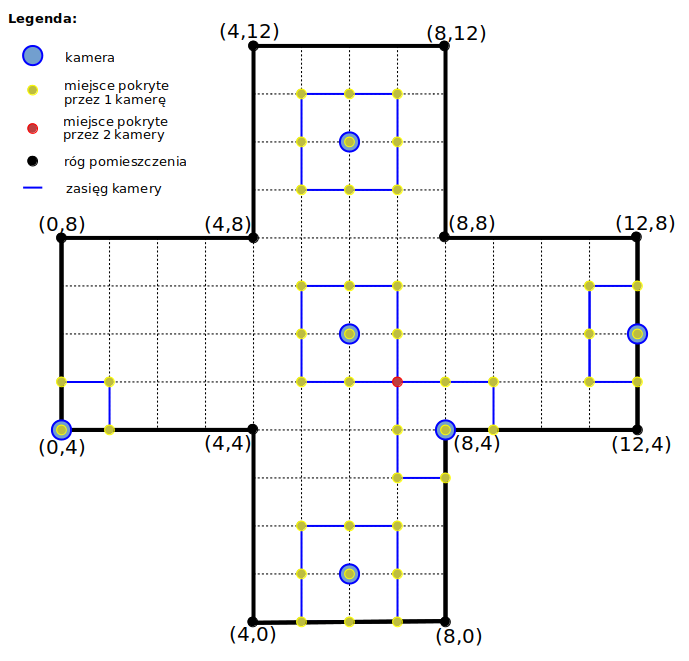
\includegraphics[scale=0.6]{img/example.png}
\end{center}


\begin{itemize}
	\item Wartości parametrów:\\
	$\alpha = 1$\\
	$\beta = 1$\\
	$r_{min} = 1$
	\item Informacje obliczone dla powyższego pomieszczenia:\\
	pole powierzchni pomieszczenia: 80\\
	$n_{kmin} = \frac{80}{2*2} = 20$\\
	$|X| = 105$
	\item Obliczenie wartości funkcji celu dla stanu z rysunku:\\
	Liczba kamer użytych: 6\\
	Pole powierzchni pokryte przez kamery: 18\\
	$p = \frac{18}{80} = 0.225$\\
	$k = \frac{max(0, 6-20)}{20} = \frac{0}{20} = 0$\\
	Parametr $r$ obliczany pierwszym sposobem:
	$r = \frac{44*0 + 61*1}{105} = \frac{61}{105} = 0.58$\\
	$f(p, k, r) = 1*0.225 - 1*0 - 1*0.58 = -0.355$\\\\
	Parametr $r$ obliczany drugim sposobem:
	$r = 1-0 = 1$\\
	$f(p, k, r) = 1*0.225 - 1*0 - 1*1 = -0.775$
\end{itemize}

\section{Metaheurystyka}
Element początkowy przestrzeni przeszukiwań jest zbiorem zawierającym $n_{kmin}$ kamer rozmieszczonych losowo wewnątrz pomieszczenia.\\
Do rozwiązania problemu użyjemy algorytmu symulowanego wyżarzania. Przy odpowiednio dobranych parametrach metoda ta, w porównaniu do algorytmów wspinaczkowych, daje większą szansę na znalezienie optymalnego rozwiązania, ponieważ zmniejsza ryzyko zatrzymania się w ekstremach lokalnych. W początkowej fazie przeszukiwania przestrzeni dopuszczalne jest przechodzenie do stanów gorszych (o mniejszej wartości funkcji celu). Wraz z rosnącą liczbą iteracji obszar poszukiwań jest ograniczany, a algorytm bardziej skupia się na poprawie bieżącego rozwiązania.

\section{Przewidywane wyniki pracy}
Przeprowadzona zostanie seria eksperymentów z różnymi wartościami parametrów $\alpha$, $\beta$, $r_{min}$ na kilku instancjach problemu (różne pomieszczenia). Dla ustalonych parametrów funkcji celu, sterować będziemy parametrami metaheurystyki, tj. funkcją wygaszania temperatury i jej
wartością początkową. Ponadto sprawdzimy dwa podejścia do zmiany położenia kamery oraz dwa sposoby obliczania parametru $r$ funkcji celu. Dla wybranej
instancji zadania sprawdzimy też wpływ gęstości siatki punktów z wnętrza
pomieszczenia na zachowanie metaheurystyki. Sporządzone zostaną wykresy przedstawiające wartość funkcji celu oraz liczbę użytych kamer w zależności od liczby wykonanych iteracji. 

\section{Implementacja}
Do realizacji zadania wykorzystaliśmy gotową implementację metaheurystyki zawartą w pakiecie simanneal w wersji 0.4.1,
której dokumentacja jest dostępna pod adresem \url{https://github.com/perrygeo/simanneal}.
Biblioteka implementuje algorytm symulowanego wyżarzania z wykładniczą funkcją wygaszania temperatury minimalizujący zadaną
funkcję celu. Z racji, że naszym zadaniem miało być maksymalizowanie opisanej w specyfikacji funkcji celu, musieliśmy zmodyfikować tę
funkcję, zmieniając jej znak na przeciwny. Poprawiony wzór na funkcję celu ma postać:
$$f(p, k, r) = - (\alpha * p - \beta * k - \frac{1}{r_{min}} * r) $$ 
Biblioteka simanneal udostępnia użytkownikowi 3 parametry, którymi można sterować zachowaniem metaheurystyki:
\begin{itemize}
\item \emph{steps} - liczba iteracji algorytmu, domyślnie 50000,
\item \emph{Tmax} - początkowa wartość temperatury, domyślnie 25000,
\item \emph{Tmin} - końcowa wartość temperatury, domyślnie 2.5.
\end{itemize}
Początkowo sprawdziliśmy zachowanie metaheurystyki dla domyślnych wartości udostepnionych parametrów, jednak
okazały się one nietrafione. 
Zmniejszyliśmy zatem temperaturę początkową 100-krotnie, czyli do wartości 250. 
W rezultacie na wykresie wartości funkcji celu względem numeru iteracji zaczęły pojawiać się charakterystyczne 
dla symulowanego wyżarzania ,,skoki'', których nasilenie zmniejszało się z kolejnymi iteracjami. 
Zaobserwowaliśmy także, że zmniejszenie liczby iteracji 2-krotnie, czyli do wartości 25000, 
nie wpłynęło na uzyskiwane rezultaty, ale za to zgodnie z intuicją zmniejszył się czas obliczeń. 
Badania postanowiliśmy zatem przeprowadzać na 25000 iteracjach.

\subsection{Plik konfiguracyjny}
Przykładowy plik konfiguracyjny wraz z komentarzami znajduje się poniżej.

\subsection{Sposób uruchomienia}

\section{Badania}
\subsection{Badanie 1}
\begin{lstlisting}
  "t_max": 250.0,
  "t_min": 2.5,
  "alpha": 10,
  "beta": 1,
  "r_min": 1,
  "num_iterations": 10000,
  "num_updates" : 100,
  "camera_move_method": "local",
  "camera_side" : 20,
  "r_count_method": "average",
  "density" : 4
\end{lstlisting}
\Figure[scale=0.4]{1/best_state.png}{Obliczony układ kamer w pomieszczeniu przez algorytm.}{label}
\Figure[scale=0.4]{1/average_costs.png}{.}{label}
zalezy nam na jak najwiekszym pokryciu, nie boli nas uzywanie kamer, dlatego jest ich duze zageszczenie.

\subsection{Badanie 2}
\begin{lstlisting}
  "t_max": 50.0,
  "t_min": 2.5,
  "alpha": 10,
  "beta": 1,
  "r_min": 1,
  "num_iterations": 10000,
  "num_updates" : 100,
  "camera_move_method": "local",
  "camera_side" : 20,
  "r_count_method": "average",
  "density" : 4
\end{lstlisting}
Zostało 

\subsection{Badanie 3}

\begin{lstlisting}
  "t_max": 50.0,
  "t_min": 2.5,
  "alpha": 10,
  "beta": 1,
  "r_min": 1,
  "num_iterations": 10000,
  "num_updates" : 100,
  "camera_move_method": "random",
  "camera_side" : 20,
  "r_count_method": "average",
  "density" : 4
\end{lstlisting}
\Figure[scale=0.4]{3/best_state.png}{Obliczony układ kamer w pomieszczeniu przez algorytm.}{label}
\Figure[scale=0.4]{3/average_costs.png}{.}{label}


\end{document}